 \documentclass[english,a4paper,12pt]{article}
\usepackage{amsmath}
\usepackage{amsfonts}
\usepackage[usenames,dvipsnames]{xcolor}
\usepackage{amssymb}
\usepackage{graphicx}
\graphicspath{ {figure/} }
\usepackage{url}
\usepackage{natbib}
\usepackage{fullpage}
\usepackage{dcolumn}
\usepackage{float}
\usepackage{caption}
\usepackage[colorlinks=true, hypertexnames=true, linkcolor=blue, citecolor=blue, urlcolor=blue]{hyperref}
\usepackage[english]{babel}
\usepackage{pdflscape}
\usepackage{rotating}
\usepackage{dcolumn}
\usepackage{blkarray}
\usepackage{eurosym}
\usepackage{longtable}
\usepackage[]{multirow}
\usepackage{csquotes}
\usepackage{epstopdf}
\usepackage{soul}
\usepackage{float}
\usepackage{rotfloat}
\usepackage{subcaption}
\usepackage{parskip}
\usepackage{enumitem}
\usepackage{placeins}
\usepackage{tikz}
\usetikzlibrary{arrows,automata,positioning, fit, calc}
\tikzset{
    state/.style={
           rectangle,
           rounded corners,
           draw=black, very thick,
           minimum height=2em,
           inner sep=4pt,
           text centered,
           },
}
\usepackage[T1]{fontenc}
\usepackage{etoolbox}
\usepackage[title]{appendix}
\setlength\parindent{0pt}
\newcommand{\dd}[1]{\mathrm{d}#1}
\renewcommand{\subfloat}[2][need a sub-caption]{\subcaptionbox{#1}{#2}}
\makeatletter
% make numeric styles use name format
\patchcmd{\NAT@test}{\else \NAT@nm}{\else \NAT@nmfmt{\NAT@nm}}{}{}
% define \citepos just like \citet
\DeclareRobustCommand\citepos
  {\begingroup
   \let\NAT@nmfmt\NAT@posfmt% ...except with a different name format
   \NAT@swafalse\let\NAT@ctype\z@\NAT@partrue
   \@ifstar{\NAT@fulltrue\NAT@citetp}{\NAT@fullfalse\NAT@citetp}}
\let\NAT@orig@nmfmt\NAT@nmfmt
\def\NAT@posfmt#1{\NAT@orig@nmfmt{#1's}}
\makeatother

\makeatletter
\AtBeginDocument{%
  \expandafter\renewcommand\expandafter\subsection\expandafter
    {\expandafter\@fb@secFB\subsection}%
  \newcommand\@fb@secFB{\FloatBarrier
    \gdef\@fb@afterHHook{\@fb@topbarrier \gdef\@fb@afterHHook{}}}%
  \g@addto@macro\@afterheading{\@fb@afterHHook}%
  \gdef\@fb@afterHHook{}%
}

\patchcmd{\maketitle}{\@fnsymbol}{\@arabic}{}{}
% \patchcmd{\maketitle}{\setcounter{footnote}{0}}{}{}{}
\makeatother

\makeatletter
\pgfdeclaregenericanchor{top base}{%
  \csname pgf@anchor@#1@north\endcsname
  \pgf@anchor@generic@top@base@main
}
\pgfdeclaregenericanchor{top base west}{%
  \csname pgf@anchor@#1@north west\endcsname
  \pgf@anchor@generic@top@base@main
}
\pgfdeclaregenericanchor{top base east}{%
  \csname pgf@anchor@#1@north east\endcsname
  \pgf@anchor@generic@top@base@main
}
\def\pgf@anchor@generic@top@base@main{%
  {%
    \pgfmathsetlength\pgf@ya{\pgfkeysvalueof{/pgf/outer ysep}}%
    \advance\pgf@y-\pgf@ya
    \pgfmathsetlength\pgf@ya{\pgfkeysvalueof{/pgf/inner ysep}}%
    \advance\pgf@y-\pgf@ya
    \pgf@ya=0pt
    \pgfutil@loop
    \ifdim\pgf@y>\baselineskip
      \advance\pgf@y-\baselineskip
      \advance\pgf@ya\baselineskip
    \pgfutil@repeat
    \global\pgf@y=\pgf@ya
  }%
}
\makeatother

\usepackage{setspace}


\title{Catchy title that describes the article in a few words}
\author{Author's name\thanks{This article was presented to many important people, who provided a multitude of useful comments that helped to make it magical. All the usual disclaimers apply, and all errors or omissions are entirely my own.}
\thanks{Permanent address: MaMTEP, Department of Business and Management, Aalborg University, Fibigerstr{\ae}de 2, Aalborg East, E-mail: greatsuccess@student.aau.dk}
\thanks{As a student at Aalborg University, I declare that I have no external or internal conflicts of interest.}
\and Author number two
\thanks{Permanent address: MaMTEP, Department of Business and Management, Aalborg University, Fibigerstr{\ae}de 2, Aalborg East, email: helpfulcoauthor@student.aau.dk}}
\date{\today}

\begin{document}

\linespread{1.0}
\selectfont
\begin{titlepage}
\maketitle
\vspace{2 cm}
\begin{abstract}
\noindent
Curabitur pretium tincidunt lacus. Nulla gravida orci a odio.  nec luctus magna felis sollicitudin mauris. Integer in mauris, as suggested by \cite{baekelbeck2015, bjerg2016} number, eu nibh euismod gravida. Duis ac tellus et risus vulputate vehicula. Donec lobortis risus a elit. Etiam tempor. Ut ullamcorper, ligula eu tempor congue, eros est euismod turpis, id tincidunt sapien risus a quam. Maecenas fermentum consequat mi. Donec fermentum. Pellentesque malesuada nulla a mi. Duis sapien sem, aliquet nec, commodo eget, consequat quis, neque. Aliquam faucibus, elit ut dictum aliquet, felis nisl adipiscing sapien, sed malesuada diam lacus eget erat. Cras mollis scelerisque nunc. Nullam arcu. Aliquam consequat. Curabitur augue lorem, dapibus quis, laoreet et, pretium ac, nisi. Aenean magna nisl, mollis quis, molestie eu, feugiat in, orci. In hac habitasse platea dictumst.
\end{abstract}

\begin{flushleft}
\small{
\vspace{2cm}


\textbf{JEL codes:} E12, E40, E51, E31.? Not necessary for a project, but they look cool.

\vspace{1cm}
\textbf{Keywords:} Fancy-topic, subtopic-excellence, critical-connection.
}
\end{flushleft}
\end{titlepage}

\linespread{1.5}
\selectfont

\section{Introduction} \label{sec:intro}

Pretty much all of the information you need to build a document in Overleaf can be found through their very user friendly help section at \url{https://www.overleaf.com/learn/how-to/Creating_a_document_in_Overleaf}.

These random words that you see below are called "ipsum lorem", and you can read about them at this interesting \href{https://en.wikipedia.org/wiki/Lorem_ipsum}{Wikipedia link}  which uses the 'hyperref' package.

Superscript in text, for a date 9\textsuperscript{th}

Donec fermentum. Pellentesque malesuada nulla a mi. Duis sapien sem, aliquet nec, commodo eget, consequat quis, neque. Aliquam faucibus, elit ut dictum aliquet, felis nisl adipiscing sapien, sed malesuada diam lacus eget erat. Cras mollis scelerisque nunc. Nullam arcu. Aliquam consequat. Curabitur augue lorem, dapibus quis, laoreet et, pretium ac, nisi. Aenean magna nisl, mollis quis, molestie eu, feugiat in, orci. In hac habitasse platea dictumst.

WOW! Just look at Figure \ref{fig:Chick-orthodox}. Is a great way to automatically include your figure numbers in your text, without having to figure out what the actual number is yourself. You will see that the "\textbackslash label:Chick-orthodox" line in the figure below is used to reference that object. And to be able to type a "\textbackslash " in regular text you have to write \textbackslash textbackslash - which is a bit of a pain, but the \textbackslash is used to control all the commands in LaTeX so it is an unfortunate necessity.

Whenever you note a fact, you will always need to reference where you got it from. If you make a statement about how something works, or what the truth about a situation is, you also need to explain who was able to show it, or how you are able to show it (i.e. refer to the evidence). to do this you need to refer to literature or data etc.

It could just be an argument that has been made by several people \citep{bell2001role,wray2006}.

Or by just one person, for example, we could note that \citet{stone1966} was one of the early researchers to help develop the United Nations National Accounts.

Or if you use a direct quote, or a reference from a book, you will also need to include the page number. For example, \citet[p.~150]{chickdow2002} noted that orthodox economic methodology is not necessarily the most appropriate to use for economic analysis, where so many of the issues are normative.

\citepos{zezza2004circuit} article can be referenced as in possessive terms (i.e. his article)

\begin{figure}
    \centering
    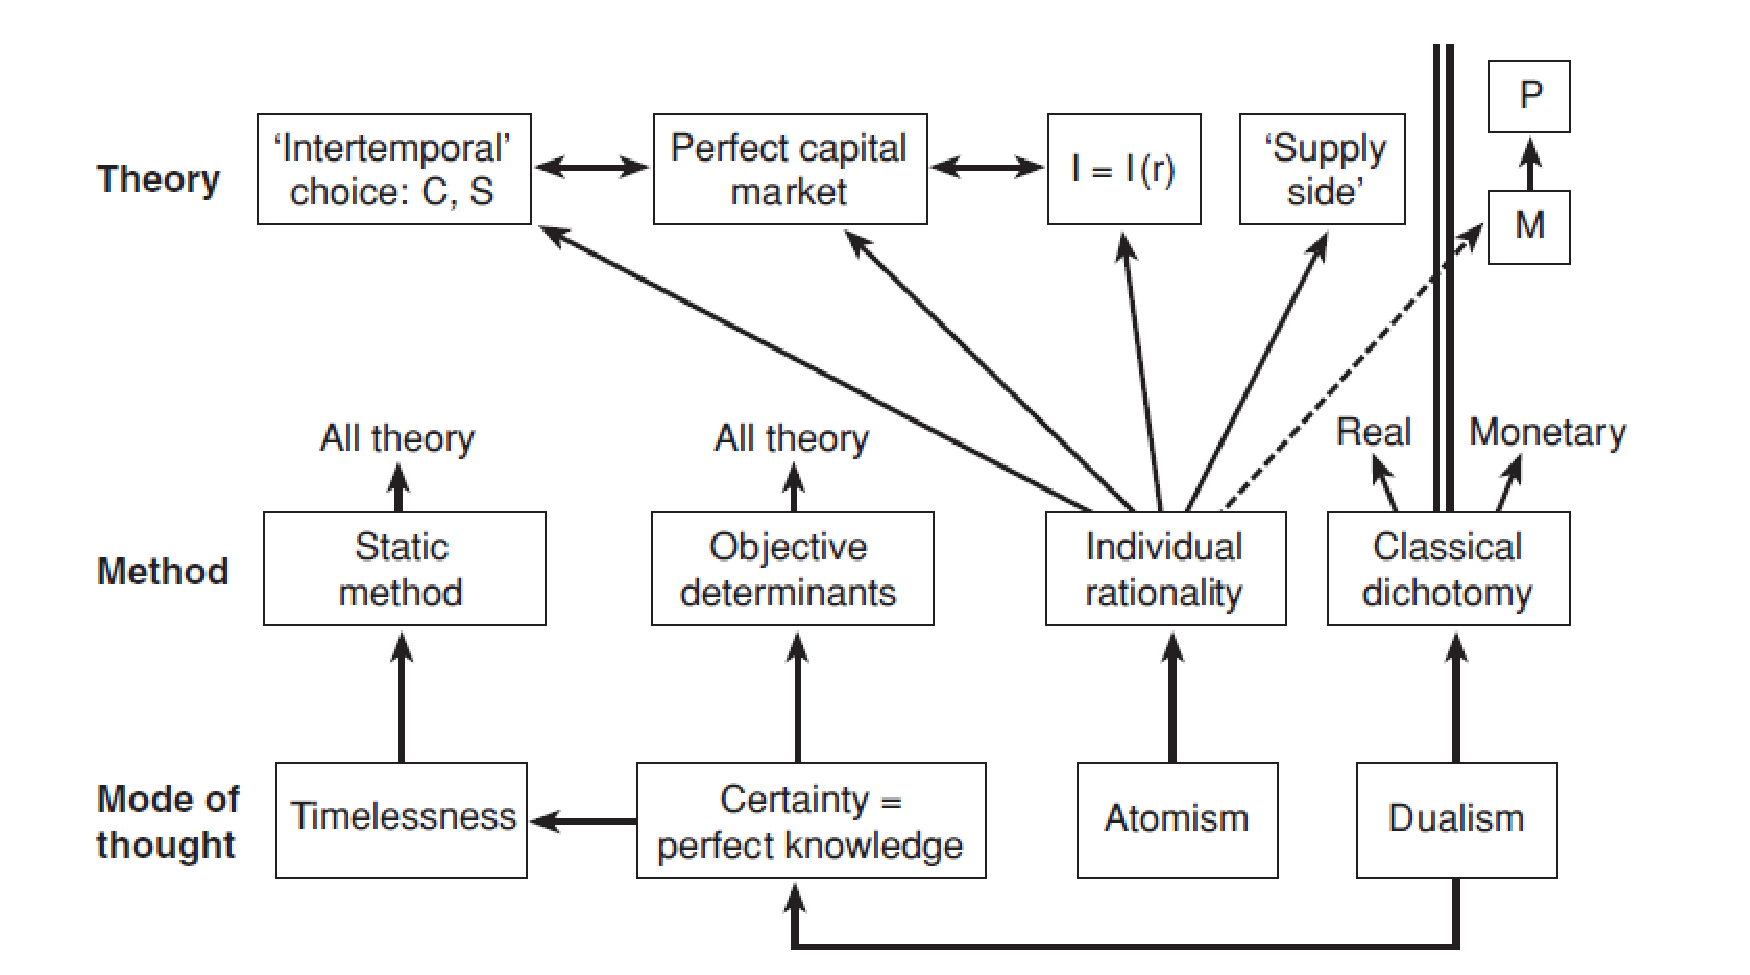
\includegraphics[width=0.9\textwidth]{images/chick2003modeofthought.pdf}
    \caption{Mode of thought}
    \label{fig:Chick-orthodox}
\end{figure}

\textbf{This is really bold font, that you might want to emphasise.}

This is a new reference for \cite{khalilkinsella2015}, and if you want it to be possessive you can use citepos \citepos{khalilkinsella2015}.

My new reference that I just added from google scholar is included \citep[p.~75]{malkiel1989efficient}.

You can also insert a "page break" using the "newpage" command.. like this: \textbackslash newpage

\newpage
Donec fermentum. Pellentesque malesuada nulla a mi. Duis sapien sem, aliquet nec, commodo eget, consequat quis, neque. Aliquam faucibus, elit ut dictum aliquet, felis nisl adipiscing sapien, sed malesuada diam lacus eget erat. Cras mollis scelerisque nunc. Nullam arcu. Aliquam consequat. Curabitur augue lorem, dapibus quis, laoreet et, pretium ac, nisi. Aenean magna nisl, mollis quis, molestie eu, feugiat in, orci. In hac habitasse platea dictumst.
 \citep{chick2003}
Donec fermentum. Pellentesque malesuada nulla a mi. Duis sapien sem, aliquet nec, commodo eget, c Aliquam consequat. Curabitur augue lorem, dapibus quis, laoreet et, pretium ac, nisi. Aenean magna nisl, mollis quis, molestie eu, feugiat in, orci. In hac habitasse platea dictumst.\footnote{This is just a footnote.}

\emph{I really really want to emphasise this text with italics}

\subsection{The subsection is available if you need it}

Sometimes you want to include a really important piece of text, as a quote from a specific author. This is a bad habit and you should really be writing what the other author has said in your own words. but just in case here is a long quote:

\begin{quote}
``Adam Smith's position depends on the truth of the proposition that, if
the baker or the brewer wants meat from the butcher, but has (the latter
being sufficiently supplied with bread and beer) nothing to offer in
exchange, no exchange can be made between them.'' \ldots{} ``Assuming
the baker and the brewer to be honest men, and honesty is no modern
virtue, the butcher could take from them an acknowledgement that they
had bought from him so much meat, and all we have to assume is that the
community would recognise the obligation of the baker and the brewer to
redeem these acknowledgements in bread or beer at the relative values
current in the village market, whenever presented to them, and we at
once have a good and sufficient currency. A sale, according to this
theory, is not the exchange of a commodity for intermediate commodity
called the''medium if exchange," but the exchange of a commodity for a
credit."
\end{quote}

\subsubsection{If you need to extend into a further sub-subsection}

When you try to compartmentalise all of your text in sub-sub-sub-sub sections it becomes more difficult to read. So if you can avoid going into too many subsections it makes the reader's job a bit easier.

\section{The next main section just needs a section command}

In this section we will insert some rather complex equations. You will notice that LaTeX really cleverly numbers the equations for you. Just as you could for the Figure above, you can also refer to you equations by their labels (and get LaTeX to create the number for you).

As in .. wow... Equation (\ref{eq:Yht}) is quite a long equation.

They could be really simple:

\begin{equation}
YD^H_t = Y^H_t - T^H_t
\end{equation}

Or they could be really complex, for example, sometimes they don't fit all in one line, and you need to break them up:

\begin{equation}
\begin{split}
Y^H_t = & WB^H_t + B2^H_{t} + r^H_{A_{t-1}}(IBA^H_{t-1})\\
        & - r^H_{L(FI)_{t-1}}(IBL(FI)^H_{t-1})\\
        & - r^H_{L(FL)_{t-1}}(IBL(FL)^H_{t-1})\\
        & + \chi _t(EQA^H_{t-1}) + \psi _t(PENA^H_{t-1}) + STR^H_t + \epsilon ^H
\label{eq:Yht}
\end{split}
\end{equation}

Sometimes you also want to have fractions in your equations, and those can also be automatically created using the "frac" command, like this:

\begin{equation}
yd^H_t = \frac{YD^H_t}{P^c_t}
\end{equation}

One of the neatest things about LaTeX is that it generates a bibliography for you automatically.

\newpage
\linespread{1}
\bibliographystyle{agsm}
\bibliography{bibliography}

\end{document}
